\documentclass[10pt,a4paper]{article}
\usepackage{listings}
\usepackage{hyperref}
\usepackage{graphicx}
\usepackage{float}
\usepackage{placeins}
\usepackage{subcaption}
\usepackage{cleveref}
\usepackage{booktabs}
\newcommand{\acomment}[1]{{\bf{\color{blue}{{[Aman: #1]}}}}}
\newcommand{\scomment}[1]{{\bf{\color{blue}{{[Suyash: #1]}}}}}

\hypersetup{
colorlinks=true,
allcolors=blue,
}

\usepackage{geometry}
\geometry{
a4paper,
% left=25mm,
% right=25mm,
top=30mm,
% bottom=30mm,
}

\title{Technical Requirements}
\author{Software Development Club, IIT Delhi}

\begin{document}


\maketitle
\section{Overview}
DevClub is the software development club of IIT Delhi with an aim to foster software development culture in the institute. It provides a platform for students who are passionate about technology to explore the field. The club has two main objectives. The first goal is to form a body of passionate students, who would use their skills to develop solutions for real problems at IIT Delhi and beyond. The second goal is to spread the knowledge that they acquire to the uninitiated, so that more and more people take part in development.
\section{Our Contribution}
Our club has an enthusiastic team of 20 students at present from different entry years.
\begin{itemize}
    \item \textbf{Team and Project Management}: An internal project and team management tool where members of the club can see progress of projects, track deadlines for tasks assigned to them, rate each other considering their performance over the last time period. It helps us manage our functioning in a streamlined manner.
    \item \textbf{File Send}: The aim of this project is to enable users to send large files seamlessly through in-browser p2p connection using WebRTC, without the hassle of uploading it on a cloud service provider like Google Drive first. It works on the browser and does not need any sharing of IPs or passwords to function.
    \item \textbf{Citadel}: Previously known as the Study Portal, Citadel was the first major project of DevClub. It is a crowd contributed platform to share study resources like lecture-notes, tutorial sheets, past question papers and other similar stuff. There is an approval process to monitor the content uploaded on the portal. It also has a fast search implemented, which enables users to search from about 3000 files.
    \item \textbf{Yearbook}: We made an online portal where the graduating students write comments about their batch mates, answer some questions about themselves and in the end they take away the Yearbook which is made from responses of all the people in their year. This acts as a memory which would always remind them about the good times they had in this institute. For example see: \href{https://devclub.in/yearbooks/ee.pdf}{EE Batch 2018 Yearbook}
    \item \textbf{Build Engine}: We have made our customized build engine that builds our projects into images and pushes them to dockerhub for general public use (which aligns with our open-source philosophy).
    \item \textbf{Slack Bot}: We have made our slack bot that manages our chat channels for different projects. It is integrated with our Team management, Build Engine and GitHub. This allows us to have a one click deploy pipeline for all our projects.
    \item \textbf{CampusBot}: CampusBot is a chatbot, which we have deployed on facebook messenger. People use it to get details about all sorts of things happening at IITD.
\end{itemize}

\section{Network Requirement}
\subsection{Overview}
For the sustenance of our club we need our VM (hosted on Baadal with IP \texttt{10.17.6.85}) to be accessible through public internet, as well as a white-listed proxy that allows us to make connections to external web.
\FloatBarrier
\begin{figure}[ht]
    \centering
    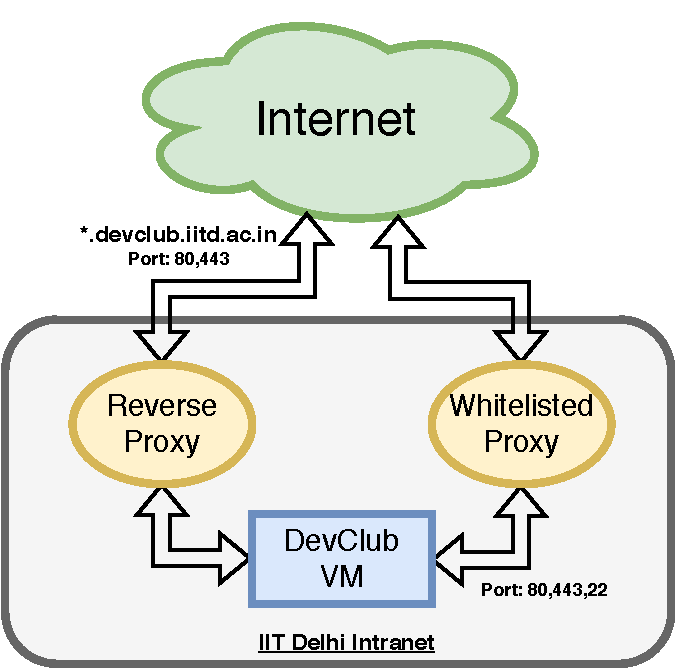
\includegraphics[width=0.6\textwidth]{architecture.pdf}
    \caption{Network Architecture \label{fig:network}}
\end{figure}
\FloatBarrier
\subsection{Reverse Proxy}
Reverse Proxy is essential since it allows users from public internet to access our services. Some of the use cases are:
\begin{itemize}
    \item \textbf{Main Website}: Build a public outreach through our main website. It needs to be publicly accessible to popularize the club and its projects.
    \item \textbf{File Send}: Many times people want to share file while using public internet and thus this needs to be publicly accessible
    \item \textbf{Campus Bot}: This requires a webhook to be accessible from public internet in order to be able to reply to messages sent through facebook and telegram.
    \item \textbf{Year Book}: Many people use home internet for filling out their profile in yearbook and thus public access is a must.
    \item \textbf{Slack Bot}: This too requires a webhook to be accessible from public internet in order to communicate with slack servers.
    \item \textbf{Build Engine}: This requires a incoming webhook to trigger the build process.
    \item \textbf{Team Management Portal}: This portal needs to be publicly accessible as it is linked with our main website and shares database across projects.
\end{itemize}
\subsection{White-listed Proxy}
White-listed Proxy is essential for us to make connection to a variety of external services. Some of the use-cases are:
\begin{itemize}
    \item \textbf{Build Engine}: This requires a connection to push the built images to the public image registry so that the whole community could use our pre-built images. Also, during the build process, it fetches various other images from registry as well as other miscellaneous requests needed to build the project.
    \item \textbf{Team Management Portal}: This requires net connection to send push notifications as well as for sending mails through Amazon Simple Email Service (SES).
    \item \textbf{Campus Bot \& Slack Bot}: They require a net connection to send automated texts and notifications to various chat groups.
\end{itemize}




% \section{Results and Outcomes}
% \begin{enumerate}
%     \item Citadel: We tracked the users that were using our portal. See
%     \cref{fig:study} for reference.
%     \begin{figure*}
%         \centering
%         \begin{subfigure}[ht]{0.9\textwidth}
%             \centering
%             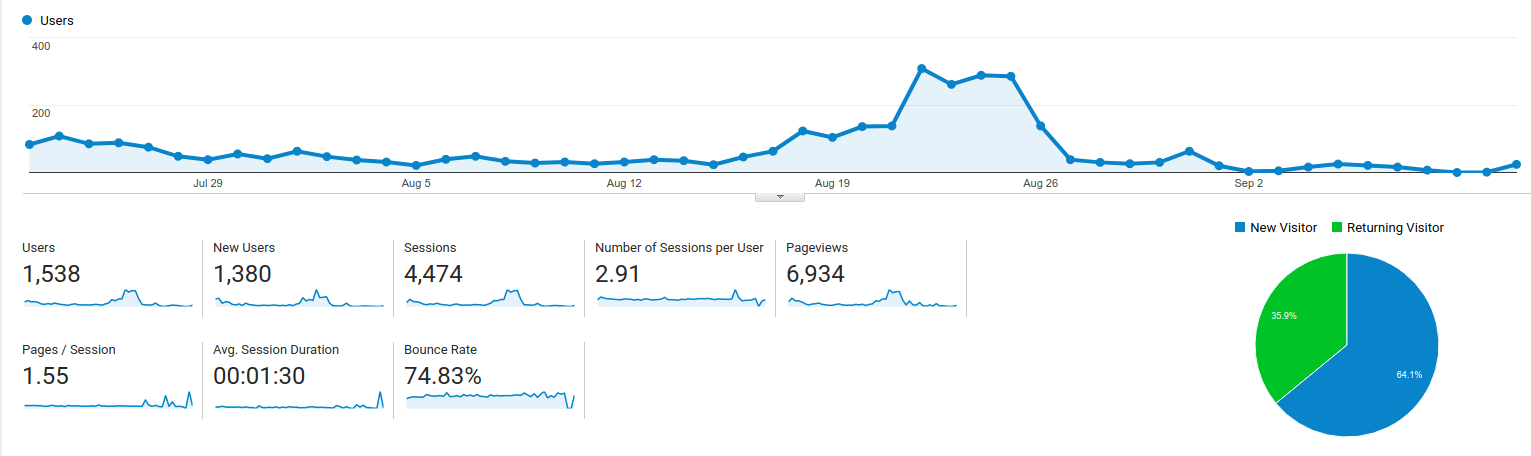
\includegraphics[width=\textwidth]{citadel.png}
%         \end{subfigure}
%         \caption{Citadel User analytics \label{fig:study}}
%     \end{figure*}
%     \item Yearbook: We tracked the users that were using our portal. See
%     \cref{fig:year} for reference.
%     \begin{figure*}
%         \centering
%         \begin{subfigure}[ht]{0.9\textwidth}
%             \centering
%             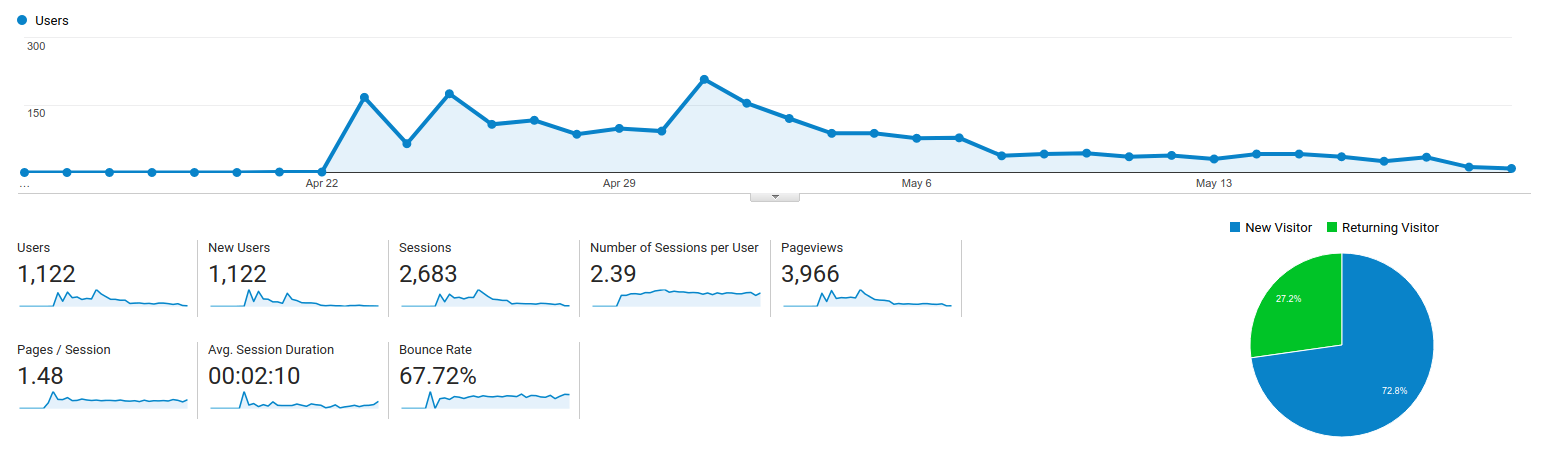
\includegraphics[width=\textwidth]{yearbook.png}
%         \end{subfigure}
%         \caption{Yearbook User analytics \label{fig:year}}
%     \end{figure*}

%     \item DevClub lectures: We take lectures on technologies like Web Development, Android Development, Git, Design Practices etc. This helps the first year students to get an idea about different technologies and they can better find their passion.
%     \item Winter Assignments: We floated some simple assignments last winter that helped students practice different technologies and frameworks they had learnt throughout the year as part of our lecture series. We were ourselves surprised by the amount of submissions we received.
%     \item Most importantly, people see us as a group they can lean on to when they want some tech related help. People ask us everyday to build something for them, but due to lack of more members and funds, we cannot help everyone. We hope that one day our club is big enough to satisfy everyone's needs.
% \end{enumerate}


% Respected Sir,

% Devclub requires access to public facing reverse proxy and a whitelisted proxy.

% The necessary details are:
% Prof. Incharge: Rijurekha Sen
% Baadal VM: 10.17.6.85 (8 Core, 8 GB Ram, 300GB HDD, Ubuntu 16.04)
% Reverse Proxy: *.devclub.iitd.ac.in, devclub.iitd.ac.in with ports 80,443
% Whitelisted Proxy: Ports 80,443 for HTTP connections, Port 22 for ssh connection

% We have attached a report stating the required architecture and need of it.

% Please do consider our request and grant us the requested resources as they are essential for continued functioning of the club. 


\end{document}